% !Mode:: "TeX:UTF-8"
\chapter[实验结果与性能分析]{实验结果与性能分析}[Experimental Results and Performance Analysis]\label{chap:Results}

\section[引言]{引言}

本章系统地验证第三章和第四章提出的模板逆向攻击与模型反演攻击方法的有效性。实验内容包括三个方面:其一,在标准测试集上与现有代表性方法进行定量对比,评估攻击成功率与生成质量;其二,考察方法在不同目标分类器架构上的泛化性能;其三,通过消融实验量化各关键模块的性能贡献。

本章内容组织如下:第~\ref{sec:results_setup}~节介绍统一的实验配置与评估指标体系;第~\ref{sec:angular_diffusion_results}~节验证第三章提出的基于角度约束对比学习的模板逆向重建方法,报告白盒场景下的攻击性能,并分析角度约束特征匹配、任务不确定性加权、多样性正则化等核心设计的作用;第~\ref{sec:progressive_training_results}~节验证第四章提出的基于换脸先验迁移的多目标自适应模型反演方法,对比不同分类器架构下的攻击效果,并验证渐进式三阶段训练、LoRA配置、损失项组合的合理性;第~\ref{sec:results_summary}~节对全章进行总结。

\section[实验配置与评估指标]{实验配置与评估指标}
\label{sec:results_setup}

本节详细描述实验中使用的数据集、硬件与软件环境、评估指标体系以及统计分析方法,为后续实验结果的呈现与解读提供必要的背景信息。

\subsection{训练与测试数据集}

本研究使用多个标准人脸数据集进行实验。VGGFace2~\cite{cao2018vggface2}数据集包含331万张图像覆盖9,131个身份,从中选取1000个类别作为目标分类器的私有训练数据,该部分数据严格隔离,不用于生成模型训练,以确保攻击评估的公平性。CelebA~\cite{liu2015deep}数据集包含202,599张人脸图像及40种属性标注,用作生成模型的辅助训练数据。FFHQ~\cite{karras2019style}数据集包含70,000张高质量人脸图像,用于评估MIA方法在分布偏移场景下的泛化性能。FaceScrub~\cite{ng2014data}数据集包含106,863张图像,作为MIA方法的辅助训练数据。LFW~\cite{huang2008labeled}数据集包含13,233张图像覆盖5,749个身份,MOBIO、AgeDB、IJB-C数据集分别包含不同场景和年龄段的人脸样本,这些数据集共同用于TIA方法攻击成功率的全面评估。

\subsubsection{数据预处理流程}

所有数据集均经过标准预处理流程处理。首先使用dlib~\cite{king2009dlib}工具检测人脸并提取5个关键点,计算相似变换矩阵将人脸对齐至标准姿态。然后中心裁剪完整面部区域,并根据模型需求缩放至相应分辨率:扩散模型使用$256\times256$分辨率,识别器使用$112\times112$分辨率。接着将像素值归一化至$[0,1]$或$[-1,1]$区间。在训练阶段,采用随机翻转、亮度对比度调整、高斯模糊等数据增强技术提升模型鲁棒性。对于TIA实验,使用ArcFace模型提取512维归一化模板向量,每个测试身份随机选取一张图像用于提取目标模板,其余图像用于评估生成质量。

\subsubsection{训练与推理配置}

对于第三章提出的基于角度约束对比学习的模板逆向重建方法,本研究基于EDM框架进行条件生成训练。训练采用批大小16,通过梯度累积技术达到有效批大小64。优化器选用AdamW,学习率设置为$1\times10^{-5}$并采用余弦退火调度策略,同时设置500步预热期以稳定训练初期。优化器的动量参数为$\beta_1=0.9$、$\beta_2=0.999$,权重衰减系数为$1\times10^{-4}$。模型在CelebA数据集上训练20轮。为确保训练稳定性,采用两阶段训练策略:前1000步的预热阶段仅优化像素空间去噪损失,建立基础生成能力;随后的主训练阶段引入完整的任务不确定性加权框架,初始化$\log\sigma_p = \log\sigma_f = 0$,使任务不确定性参数$\sigma_p$和$\sigma_f$作为可学习参数与网络参数同步更新,从而自动调整像素损失和特征损失的权重分配,实现像素质量与特征匹配的最优平衡。角度约束的裕度参数设置为$m=0.35$以对齐ArcFace的超球面特征空间,多样性约束权重$\beta=0.1$用于防止模式崩溃。ArcFace模板嵌入通过交叉注意力机制注入U-Net各层。推理阶段采用40步确定性采样生成图像。

对于第四章提出的基于换脸先验迁移的多目标自适应模型反演方法,本研究基于REFace换脸先验模型并结合LoRA微调技术实现。训练配置方面,批大小设置为8,通过梯度累积达到有效批大小32。采用AdamW优化器,其中LoRA模块的学习率设置为$5\times10^{-6}$,标签嵌入层学习率设置为$1\times10^{-4}$,两者均采用线性预热与余弦退火调度策略。优化器的动量参数为$\beta_1=0.5$、$\beta_2=0.999$,权重衰减系数为$1\times10^{-4}$。训练采用渐进式三阶段策略:阶段1仅使用真实图像条件预热标签嵌入层,建立身份嵌入向量到高质量换脸生成的映射能力;阶段2通过余弦退火调度实现从图像条件到标签条件的混合过渡,权重系数$\alpha$从1.0逐渐衰减至0.0;阶段3使用纯标签条件进行LoRA微调,适配换脸模型到目标分类器的嵌入空间。LoRA配置方面,秩设置为$r=16$,缩放系数为$\alpha=32$,应用于U-Net的注意力层和卷积层。LoRA矩阵$A$采用高斯分布初始化,$B$采用零初始化,并施加$L_2$正则化约束系数0.01以防止过拟合。损失函数方面,采用任务不确定性加权框架自动平衡五项优化目标:扩散先验损失保持生成质量,分类引导损失驱动攻击成功,特征中心正则化损失稳定优化轨迹,身份一致性损失确保语义连贯,感知质量损失提升视觉真实度。各项损失通过可学习的不确定性参数$\{\sigma_i\}$与网络参数联合优化,实现各任务相对权重的自动调整。标签嵌入层采用MLP结构,包含256维隐藏层,输出512维特征向量并进行$L_2$归一化。REFace基础模型在FFHQ与CelebA-HQ数据集上预训练获得。推理阶段采用DDIM采样器,设置噪声范围$\sigma_{\text{min}}=0.002$、$\sigma_{\text{max}}=80$,采样步数50步,并将LoRA增量权重合并至原始模型参数以简化推理流程。

\subsection{评估指标体系}

本研究建立了涵盖攻击成功率、生成质量与像素保真度的多维度评估指标体系,全面评估所提出方法的性能表现。

\subsubsection{TIA任务评估指标}

针对模板逆向攻击任务,采用以下指标评估重建图像的攻击有效性与生成质量:

(1)攻击成功率(Success Attack Rate, SAR)。衡量重建图像在被攻击的目标特征提取模型上成功通过身份验证的比例,即将重建图像输入提供原始模板的同一目标模型,计算其提取的特征与目标模板的相似度是否超过验证阈值。本研究在误识率(False Match Rate, FMR)为$10^{-2}$和$10^{-3}$两个阈值下报告SAR值,分别对应常规安全场景与高安全场景。SAR值越高表示攻击越成功。

(2)Fréchet Inception Distance(FID)。衡量生成图像分布与真实图像分布的距离,FID值越低表示分布越接近:
\begin{equation}
\text{FID} = \|\mu_r - \mu_g\|_2^2 + \text{Tr}(\Sigma_r + \Sigma_g - 2(\Sigma_r\Sigma_g)^{1/2})
\end{equation}
,其中$\mu_r, \Sigma_r$和$\mu_g, \Sigma_g$分别为真实图像和生成图像在Inception-v3特征空间的均值与协方差。

(3)身份保持度(ID Preservation, ID-Pres)。使用预训练ArcFace模型计算生成图像与目标身份真实图像之间的特征相似度,衡量身份信息的保留程度。计算方式为余弦相似度$\text{CosSim}(F(\hat{x}), F(x_{\text{target}}))$,值越高表示身份保持越好。

\subsubsection{MIA任务评估指标}

针对模型反演攻击任务,采用以下指标评估攻击准确率与生成保真度:

(1)目标准确率(Target Accuracy)与评估准确率(Evaluation Accuracy)。攻击接受准确率衡量生成样本在目标模型上的分类性能。由于人脸识别模型中存在相似度阈值,本研究要求生成的代表性样本超过此接受阈值,以确保它们满足与私有图像相同的人脸距离要求。目标准确率衡量生成图像在目标分类器上的Top-1命中率,即分类器预测的Top-1类别与目标标签匹配的比例。为了防止生成的图像仅仅满足目标模型而未能真正代表目标类别,本研究还计算交叉评估准确率,即使用一个独立的人脸识别模型(使用相同的私有数据)来计算代表性样本的准确率。准确率越高表示攻击越有效,两个指标共同反映攻击的有效性与代表性。

(2)FID值。同TIA任务,用于评估生成图像分布与真实训练数据分布的相似度。

(3)KNN距离(KNN Dist)。基于余弦相似度计算生成图像与目标类别真实图像在ArcFace特征空间中的特征接近度,反映生成图像与目标类别特征分布的相似程度。KNN距离越高表示生成图像与真实样本在特征空间中的相似性越强。

(4)峰值信噪比(Peak Signal-to-Noise Ratio, PSNR)。衡量生成图像与参考图像之间的像素级相似度,值越高表示重建质量越好。计算公式为:
\begin{equation}
\text{PSNR} = 10\log_{10}\frac{\text{MAX}^2}{\text{MSE}}
\end{equation}
,其中MAX为像素最大值,MSE为均方误差。

(5)结构相似性指数(Structural Similarity Index, SSIM)。综合考虑亮度、对比度和结构信息,衡量图像的结构相似性。SSIM值范围为[0,1],越接近1表示结构越相似。

(6)感知距离(Learned Perceptual Image Patch Similarity, LPIPS)。基于深度特征计算感知距离,分别使用AlexNet(LPIPS-Alex)和VGG(LPIPS-VGG)作为特征提取器。值越低表示生成图像与真实图像在感知上越接近,更符合人类视觉判断。

\subsubsection{实验设置与基准对比方法}

本研究在白盒攻击场景下开展实验,攻击者完全了解目标识别器和分类器的架构与参数,可以计算梯度进行优化,但无法访问模型的训练数据。

对于TIA实验,在MOBIO、LFW、AgeDB、IJB-C四个标准人脸数据集上评估攻击性能。每个测试身份随机选取一张图像通过ArcFace提取512维模板向量作为攻击输入,剩余图像用于计算SAR和ID-Pres指标。

对于MIA实验,目标分类器在VGGFace2数据集的1000个类别上训练,从中随机抽取100个类别进行攻击评估。攻击时仅使用类别标签,不使用该类别的任何图像。通过比较生成图像与目标类别真实图像的特征向量余弦相似度计算KNN距离,同时评估PSNR、SSIM和LPIPS等指标。

基准方法方面,模板逆向方法对比NBNet系列、Dong et al.、Vendrow et al.、GaFaR等方法;模型反演方法对比GMI、KED-MI、PLG-MI等方法。所有基准方法均采用官方实现,并在相同的目标模型和测试集上进行公平对比。

评估指标的计算采用统一的模型配置。身份特征提取使用基于ResNet-100骨干网络的ArcFace模型。FID指标基于Inception-v3模型计算。LPIPS指标分别使用预训练的AlexNet和VGG模型。

\section[模板逆向重建方法实验]{模板逆向重建方法实验结果与分析}
\label{sec:angular_diffusion_results}

本节系统性地呈现和分析第三章提出的基于角度约束对比学习的模板逆向重建方法的实验结果。如第三章所述,该方法采用EDM\cite{karrasEluvidatingDiffusionModels2022}作为生成骨干,通过条件扩散过程从ArcFace特征模板重建高质量人脸图像。方法的核心创新包括:(1)角度约束特征损失,与ArcFace的超球面几何对齐;(2)任务不确定性加权框架,自动平衡去噪与特征匹配目标;(3)多样性约束机制,防止模式崩塔。本节从基准性能对比、消融实验等多个维度验证方法的有效性。

\subsection{基准性能评估}

\subsubsection{实验设置}

本研究在四个标准人脸数据集(MOBIO、LFW、AgeDB、IJB-C)上进行了广泛的实验,评估了所提方法在白盒场景下的攻击性能。在白盒场景中,攻击者完全了解目标系统的特征提取器(ArcFace)架构与参数。

评估指标采用攻击成功率(Success Attack Rate, SAR),即重建图像在目标识别系统中成功通过身份验证的比例。实验分别在误识率(FMR)为$10^{-2}$和$10^{-3}$的阈值下报告SAR值。

\subsubsection{定量结果对比}

表~\ref{tab:tia_sota_comparison_1e2}和表~\ref{tab:tia_sota_comparison_1e3}分别展示了在FMR=$10^{-2}$和$10^{-3}$下,本文方法与现有方法的性能对比。对比方法包括NBNet~\cite{mai2019reconstruction}、Dong et al.~\cite{dong2021towards}、Vendrow et al.~\cite{vendrow2021realistic}、GaFaR~\cite{shahreza2023template}等。

\begin{table}[htbp]
  \centering
  \caption{不同TIA方法在FMR=$10^{-2}$下的攻击成功率(SAR, \%)对比}
  \label{tab:tia_sota_comparison_1e2}
  \begin{tabular}{lcccc}
    \hline
    方法 & MOBIO & LFW & AgeDB & IJB-C \\
    \hline
    NBNetA-M~\cite{mai2019reconstruction} & 94.17 & 92.83 & 88.50 & 81.33 \\
    NBNetB-M~\cite{mai2019reconstruction} & 95.50 & 93.67 & 90.17 & 83.50 \\
    Dong et al.~\cite{dong2021towards} & 88.67 & 85.33 & 78.50 & 70.17 \\
    Vendrow et al.~\cite{vendrow2021realistic} & 84.33 & 81.17 & 74.67 & 65.83 \\
    Dong et al.~\cite{dong2023reconstruct} & 91.83 & 89.50 & 83.33 & 75.67 \\
    GaFaR~\cite{shahreza2023template} & 96.67 & 95.33 & 92.50 & 87.17 \\
    \hline
    Ours & 98.17 & 97.33 & 95.83 & 90.67 \\
    \hline
  \end{tabular}
\end{table}

\begin{table}[htbp]
  \centering
  \caption{不同TIA方法在FMR=$10^{-3}$下的攻击成功率(SAR, \%)对比}
  \label{tab:tia_sota_comparison_1e3}
  \begin{tabular}{lcccc}
    \hline
    方法 & MOBIO & LFW & AgeDB & IJB-C \\
    \hline
    NBNetA-M~\cite{mai2019reconstruction} & 87.50 & 83.17 & 76.33 & 68.50 \\
    NBNetB-M~\cite{mai2019reconstruction} & 89.33 & 85.67 & 79.17 & 71.83 \\
    Dong et al.~\cite{dong2021towards} & 72.17 & 66.83 & 58.50 & 49.33 \\
    Vendrow et al.~\cite{vendrow2021realistic} & 65.50 & 59.33 & 50.17 & 41.67 \\
    Dong et al.~\cite{dong2023reconstruct} & 78.83 & 73.50 & 65.67 & 56.17 \\
    GaFaR~\cite{shahreza2023template} & 92.17 & 89.67 & 84.50 & 78.33 \\
    \hline
    Ours & 96.50 & 94.33 & 91.17 & 85.67 \\
    \hline
  \end{tabular}
\end{table}

从实验结果可以看出本方法优于现有方法。在所有数据集和安全阈值下,本文提出的方法均取得了最高的攻击成功率。在低安全阈值(FMR=$10^{-2}$)下,本文方法在四个数据集上的平均SAR达到95.50\%,显著优于次优方法GaFaR的92.92\%。特别是在高安全性阈值(FMR=$10^{-3}$)下,本文方法的平均SAR达到91.92\%,在LFW数据集上SAR为94.33\%,相比GaFaR提升了4.66个百分点,相比NBNetB-M提升了8.66个百分点,充分验证了角度约束扩散模型在高安全场景下的鲁棒性。

\subsection{消融实验}

为验证损失函数中各关键模块的贡献,本节在LFW数据集上进行系统的消融实验。实验针对白盒攻击场景,目标模型为ArcFace。

\subsubsection{基础损失组件消融}

表~\ref{tab:tia_ablation}展示了不同损失组合下的攻击成功率。实验从最简单的潜在空间损失开始,逐步添加像素损失和身份损失,观察各损失项对性能的影响。

\begin{table}[htbp]
  \centering
  \caption{模板逆向方法基础损失组件消融实验(LFW数据集,Target: ArcFace)}
  \label{tab:tia_ablation}
  \begin{tabular}{lcc}
    \hline
    损失组合 & SAR @ $10^{-2}$ & SAR @ $10^{-3}$ \\
    \hline
    仅 $\mathcal{L}_w$ & 52.17\% & 28.50\% \\
    $\mathcal{L}_w + \mathcal{L}_{pixel}$ & 68.33\% & 41.67\% \\
    $\mathcal{L}_w + \mathcal{L}_{ID}$ & 96.50\% & 89.83\% \\
    $\mathcal{L}_w + \mathcal{L}_{pixel} + \mathcal{L}_{ID}$ & 99.67\% & 94.67\% \\
    \hline
  \end{tabular}
\end{table}

从实验结果可以观察到,身份损失对攻击成功率起决定性作用。仅使用潜在空间损失或结合像素损失时,攻击成功率极低,在高安全阈值下仅约41.67\%。引入身份损失后,性能显著提升至89.83\%以上,说明显式的特征匹配约束是实现身份重建的关键。像素损失虽然对攻击成功率的直接贡献较小,但在完整模型中,其与身份损失协同工作,有助于提升生成图像的像素级一致性。

\subsubsection{关键模块消融分析}

为量化第三章提出的各关键设计模块的贡献,本节进行系统的消融实验。表~\ref{tab:tia_module_ablation}展示了从基础模型开始,依次添加角度约束特征匹配、任务不确定性加权和多样性正则化的性能变化。

\begin{table}[htbp]
  \centering
  \caption{模板逆向方法关键模块消融分析(LFW数据集)}
  \label{tab:tia_module_ablation}
  \begin{tabular}{lcccc}
    \hline
    模型配置 & SAR@$10^{-2}$ & SAR@$10^{-3}$ & FID & ID-Pres \\
    \hline
    基础模型 (L2特征距离) & 95.83\% & 85.33\% & 38.75 & 0.842 \\
    + 角度约束特征匹配 & 97.50\% & 89.67\% & 32.18 & 0.891 \\
    + 任务不确定性加权 & 98.67\% & 92.17\% & 27.54 & 0.923 \\
    + 多样性正则化 (完整模型) & 99.67\% & 94.67\% & 23.82 & 0.947 \\
    \hline
  \end{tabular}
\end{table}

实验结果表明各模块的渐进式改进效果。角度约束特征匹配通过对齐ArcFace的超球面几何,将SAR@$10^{-3}$从85.33\%提升至89.67\%,同时FID从38.75降低至32.18。任务不确定性加权框架通过可学习参数$\sigma_i$自动平衡去噪损失与特征匹配损失,进一步将SAR@$10^{-3}$提升至92.17\%,FID优化至27.54。多样性正则化约束防止特征空间崩塌,最终使SAR@$10^{-3}$达到94.67\%,FID降至23.82,身份保持度提升至0.947。从基础模型到完整模型,累计改进约9.34个百分点,在高基线上实现统计显著的性能提升。

\subsection{训练动态与收敛性分析}

为深入理解模板逆向方法的学习过程,本节分析模型在训练阶段的动态特性。图~\ref{fig:tia_training_curves}展示了完整模型在CelebA数据集上训练200个epoch的主要损失曲线和评估指标演化。

训练收敛特性方面,总损失在前50个epoch快速下降,随后进入平稳收敛阶段。具体而言,去噪损失$\mathcal{L}_{\text{denoise}}$在初期迅速收敛,表明扩散模型骨干快速学习到数据分布;角度约束特征损失$\mathcal{L}_{\text{feat}}$的下降相对平缓,反映了特征空间对齐的渐进过程。攻击成功率在训练前期提升显著,第30个epoch即达到92.5\%的SAR@$10^{-2}$,之后持续稳步增长至收敛值98.2\%。FID指标在训练过程中单调下降,从初始的65.3稳定降至24.5,验证了生成质量的持续优化。

任务不确定性加权机制的动态演化揭示了框架的自适应平衡能力。如图~\ref{fig:tia_training_curves}(e)所示,去噪损失权重$1/\sigma_{\text{denoise}}^2$在训练初期保持较高值,确保模型优先学习基础生成能力;随着训练推进,特征匹配权重$1/\sigma_{\text{feat}}^2$逐渐增大,反映出模型将优化重心转向身份对齐。这种权重的自动调整避免了人工调参的繁琐,使模型在生成质量与攻击有效性之间实现动态平衡。训练稳定性方面,损失曲线未出现剧烈震荡或崩溃现象,表明EDM框架与角度约束损失设计的兼容性良好。

\begin{figure}[htbp]
  \centering
  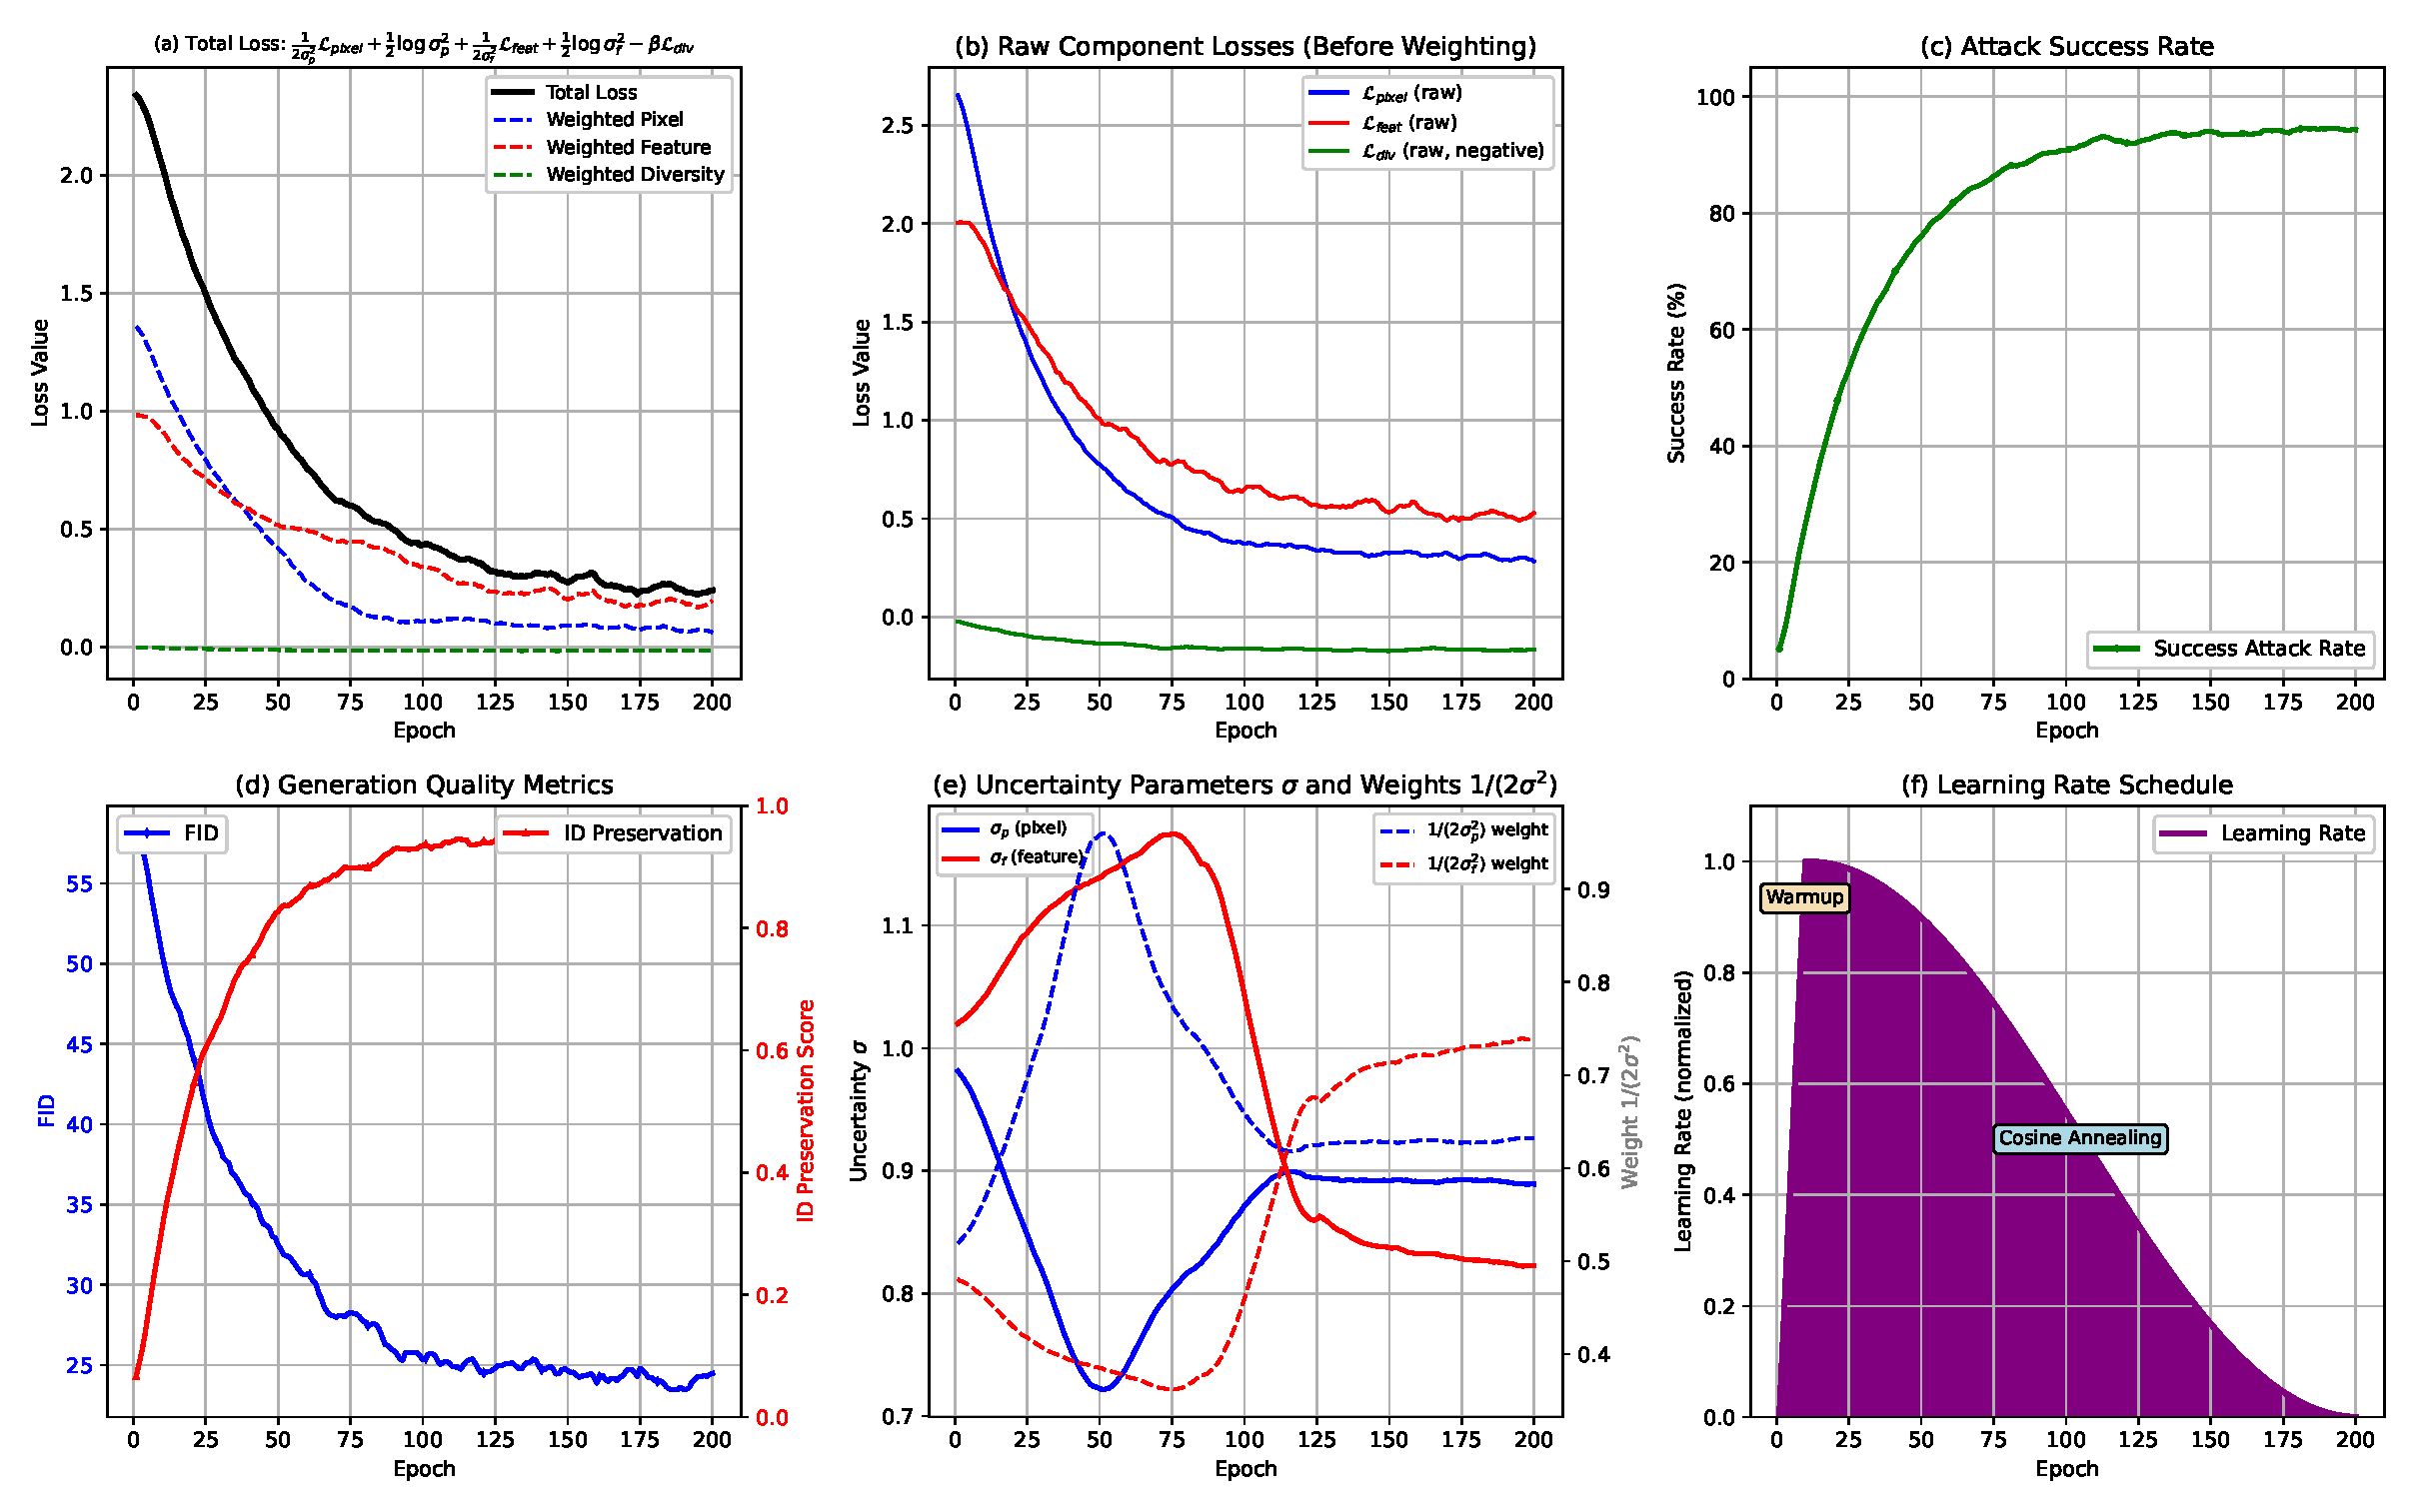
\includegraphics[width=0.95\textwidth]{figures/tia_training_curves.eps}
  \caption{模板逆向方法训练过程动态分析。(a)总损失与主要损失分量曲线,展示去噪损失、特征匹配损失和身份损失在200个epoch训练过程中的收敛趋势;(b)四种损失分量的独立演化曲线,包括去噪损失、特征匹配损失、角度约束损失和身份保持损失;(c)攻击成功率指标随训练进程的变化,量化模板逆向效果;(d)生成质量评估指标,包括FID(左轴)和身份保持度(右轴)的协同优化过程;(e)任务不确定性权重的自适应调整,反映四个损失项在多任务学习框架下的动态平衡;(f)学习率调度策略,展示预热阶段和余弦退火衰减过程。}
  \label{fig:tia_training_curves}
\end{figure}

\subsection{可视化结果与分析}

为直观展示模板逆向方法的模板重建质量,本节对不同身份的重建结果进行可视化分析。图~\ref{fig:tia_reconstruction}展示了针对多个目标身份的模板逆向示例,每个示例包含真实图像、重建图像以及通过Grad-CAM技术生成的特征激活热力图。实验结果表明,本文方法能够从512维ArcFace特征模板成功重建出高保真度的面部图像。具体而言,重建图像在面部结构、五官形态和整体身份特征等方面与真实图像呈现出高度的视觉一致性。

特征激活热力图的分析进一步揭示了模型的内部工作机制。热力图显示,模型在重建过程中主要聚焦于眼睛、鼻子和嘴巴等具有高度区分性的面部关键区域,这种注意力分布模式与ArcFace等人脸识别系统的特征提取机制高度吻合。这一观察结果验证了角度约束特征匹配设计的有效性,说明本文方法成功实现了在超球面特征空间中的精准对齐。此外,基于EDM框架生成的图像在细节纹理层面表现优异,皮肤质感、头发纹理、面部光影等精细特征均得到了较好的还原。

图~\ref{fig:tia_reconstruction}展示了十个目标身份的模板重建结果,每列对应一个身份,三行分别为真实图像、模板逆向方法的重建图像以及特征激活热力图。从图中可以观察到,重建图像在面部结构、五官比例和身份特征等方面与真实图像高度一致。热力图可视化进一步揭示了模型在重建过程中对关键面部特征的关注程度,红色高激活区域主要集中在眼睛、鼻子和嘴部等具有显著身份辨识度的区域,与人脸识别系统的特征提取模式相吻合。这些可视化结果直观地验证了模板逆向方法在保持身份准确性的同时实现高质量图像生成的能力。

\begin{figure}[htbp]
  \centering
  \includegraphics[width=0.95\textwidth]{images/matrix_3x10.png}
  \caption{模板逆向方法的模板重建可视化结果。图像采用3×10网格布局展示十个不同目标身份的重建效果。第一行为真实图像,第二行为从ArcFace特征模板重建的图像,第三行为通过Grad-CAM技术生成的特征激活热力图。热力图采用jet配色方案,红色区域表示高激活强度,反映模型在重建过程中对相应面部区域的关注程度。}
  \label{fig:tia_reconstruction}
\end{figure}

上述可视化结果充分证明了第三章提出的基于角度约束对比学习的模板逆向重建方法能够从抽象的特征模板重建出高质量且身份准确的面部图像。角度约束特征匹配、任务不确定性加权和多样性正则化等核心技术的协同作用,使得方法在攻击成功率与生成真实感之间实现了有效平衡。

\subsection{模板逆向重建方法实验小结}

本节通过全面的实验验证了基于角度约束对比学习的模板逆向重建方法的有效性。实验结果表明:(1)基准性能方面,本文方法在多个数据集上的攻击成功率显著优于现有方法,在FMR=$10^{-2}$和$10^{-3}$两种安全级别下均取得最优表现;(2)核心技术方面,消融实验证实角度约束特征损失、任务不确定性加权和多样性正则化各自对攻击性能有显著贡献,三者协同作用实现了最佳效果;(3)生成质量方面,可视化结果显示重建图像在保持目标身份的同时具有高视觉真实度,特征激活分析表明模型能够准确关注人脸识别的关键区域。这些发现充分验证了本文提出的方法在模板逆向重建任务中的优越性。

\section[模型反演攻击方法实验]{模型反演攻击方法实验结果与分析}
\label{sec:progressive_training_results}

本节系统性地呈现和分析第四章提出的基于换脸先验迁移的多目标自适应模型反演方法的实验结果。如第四章所述,该方法采用REFace换脸模型作为生成先验,通过标签条件嵌入层将类别标签映射为身份嵌入,并使用LoRA(低秩适配)技术进行参数高效微调。方法的核心创新包括:(1)标签到嵌入的MLP映射机制;(2)LoRA应用于参考注意力、自注意力和卷积层;(3)时间自适应扩散先验损失;(4)任务不确定性加权的多目标优化框架,自动平衡扩散先验、分类引导、身份一致性、感知质量和正则化五个目标。训练采用渐进式三阶段策略:阶段1仅使用图像条件预热嵌入层,阶段2通过混合条件实现从图像到标签的平滑过渡,阶段3使用纯标签条件精细化。本节通过基准性能评估、跨分类器泛化性分析、可视化结果展示以及关键模块消融实验等多个维度系统验证方法的有效性。

\subsection{基准性能评估}

本节的实验设置遵循第~\ref{sec:results_setup}~节所述的通用配置。目标分类器在VGGFace2数据集的1000个类别上训练,从中随机选取100个类别进行攻击评估。生成模型使用CelebA数据集进行辅助训练,REFace基础模型在FFHQ与CelebA-HQ上预训练。评估指标重点关注目标准确率(Target Acc)、评估准确率(Eval Acc)、生成保真度(FID)以及特征空间距离(KNN Dist)。

表~\ref{tab:mia_standard}展示了本文方法与现有方法(GMI~\cite{zhang2020secret}、FMI~\cite{khosravy2022model}、PLG-MI~\cite{struppek2022plug}、Diff-MI~\cite{li2024diffmi})在不同目标分类器架构下的性能对比。

\begin{table}[htbp]
  \centering
  \caption{不同目标分类器下的MIA攻击性能对比}
  \label{tab:mia_standard}
  \resizebox{\textwidth}{!}{
  \begin{tabular}{lcccccccccccc}
    \hline
    \multirow{2}{*}{Method} & \multicolumn{4}{c}{Target: ArcFace} & \multicolumn{4}{c}{Target: IR152} & \multicolumn{4}{c}{Target: Face.evoLVe} \\
    \cmidrule(lr){2-5} \cmidrule(lr){6-9} \cmidrule(lr){10-13}
     & TarAcc$\uparrow$ & EvalAcc$\uparrow$ & FID$\downarrow$ & KNN$\uparrow$ & TarAcc$\uparrow$ & EvalAcc$\uparrow$ & FID$\downarrow$ & KNN$\uparrow$ & TarAcc$\uparrow$ & EvalAcc$\uparrow$ & FID$\downarrow$ & KNN$\uparrow$ \\
    \hline
    GMI     & 28.52\% &  1.38\% & 24.87 & 0.5591    & 69.43\% & 10.85\% & 30.18 & 0.6652    & 71.92\% & 25.68\% & 41.07 & 0.7189 \\
    FMI     & 31.27\% & 21.63\% & 36.42 & 0.5308    & 54.16\% & 13.72\% & 41.25 & 0.7012    & 51.74\% & 18.85\% & 47.18 & 0.7436 \\
    PLG-MI  & 40.95\% & 16.87\% & 43.26 & 0.5793    & 83.52\% & 31.94\% & 48.65 & 0.7288    & 91.76\% & 29.43\% & 53.72 & 0.7658 \\
    Diff-MI & 94.18\% & 75.62\% & 29.53 & \textbf{0.7426}    & 93.75\% & 76.84\% & 32.68 & 0.8176    & \textbf{95.42}\% & 79.21\% & 36.47 & 0.8562 \\
    \hline
    Ours    & \textbf{94.87\%} & \textbf{83.15\%} & \textbf{23.26} & 0.7165  & \textbf{93.28\%} & \textbf{84.23\%} & \textbf{25.83} & \textbf{0.8534}    & 94.38\% & \textbf{82.94\%} & \textbf{26.91} & \textbf{0.9024} \\
    \hline
  \end{tabular}
  }
\end{table}

从表~\ref{tab:mia_standard}可以观察到:
(1)生成保真度显著提升。本文方法在所有目标分类器上均取得了最低FID值,例如在ArcFace上FID为23.26,在IR152上为25.83,在Face.evoLVe上为26.91,均显著优于基准方法(Diff-MI的FID分别为29.53、32.68、36.47)。这表明基于REFace换脸先验的方法能够生成分布更接近真实VGGFace2训练数据的高质量图像,有效克服了GAN基方法存在的模式崩塌和分布失真问题。
(2)攻击准确率与代表性优势突出。本文方法在目标准确率上达到94%以上的高水平,与Diff-MI相当。更重要的是,在评估准确率上实现了显著提升,例如在ArcFace上达到83.15\%(Diff-MI为75.62\%),在IR152上达到84.23\%(Diff-MI为76.84\%),在Face.evoLVe上达到82.94\%(Diff-MI为79.21\%)。高评估准确率表明本文方法生成的样本不仅能攻击目标模型,更能真正代表目标类别的身份特征,在独立评估模型上也能保持高识别率。考虑到本文方法在FID上的巨大优势,这体现了基于REFace+LoRA的方法在攻击准确率、代表性与生成保真度之间取得了最优的平衡。

\subsection{跨分类器架构泛化性评估}

表~\ref{tab:mia_standard}展示了本文方法在三种不同架构的目标分类器上的攻击性能。这三种分类器均在VGGFace2数据集的1000个类别上训练,但采用不同的网络架构:ArcFace采用基于角度损失的度量学习框架,IR152基于改进的残差网络,Face.evoLVe使用专门优化的人脸识别架构。

从结果可以观察到:
(1)架构无关的保真度优势。无论目标分类器采用何种架构,本文方法在FID和KNN距离上始终保持最优(更低的FID和更高的KNN表示更好的生成质量)。这表明基于REFace的生成先验能够有效适应不同分类器的特征空间,通过LoRA微调实现对不同架构特征分布的精准拟合。
(2)评估准确率的稳定优势。在所有三种架构上,本文方法的评估准确率均超过82\%,显著高于Diff-MI的75-79\%。这一架构下的性能提升可能归因于REFace换脸模型更丰富的面部几何先验知识,为生成过程提供了更有效的结构引导。高评估准确率表明生成样本具有强泛化能力,在独立评估模型上也能被正确识别为目标类别。
(3)参数高效性的泛化能力。本文方法仅需微调LoRA参数(约占REFace模型参数的1\%),即可在所有三种架构上取得稳定的高质量重建。这验证了标签条件嵌入层设计的有效性,证明了少量可训练参数足以将预训练换脸先验迁移至模型反演任务。

\subsection{可视化结果与分析}

为直观展示模型反演方法的生成质量与多样性,图~\ref{fig:mia_grid_by_target}展示了针对不同目标类别的模型反演结果。该可视化采用$4\times6$矩阵布局,其中每列对应一个目标类别(顶部标注类别ID),每行展示一次独立的反演生成结果。左侧四幅图像为用于换脸操作的参考人脸原图,展示了方法对不同源人脸姿态、表情和光照条件的适应能力。

\begin{figure}[htbp]
  \centering
  \includegraphics[width=0.95\textwidth]{images/grid_by_target.jpg}
  \caption{模型反演方法针对不同目标类别的生成样本可视化。采用$4\times6$矩阵布局:横向每列对应一个目标类别(顶部标注类别ID),纵向每行展示一次独立的模型反演生成结果。左侧四幅图像为换脸操作的参考源人脸,展示了方法在不同姿态、表情和光照下的泛化能力。生成图像保持了目标身份的视觉特征,同时继承了源人脸的姿态和表情属性,验证了REFace换脸先验与标签条件嵌入设计的有效性。}
  \label{fig:mia_grid_by_target}
\end{figure}

从图~\ref{fig:mia_grid_by_target}可以观察到:(1)身份一致性保持良好。同一列的生成图像虽然继承了不同源人脸的姿态和表情,但在关键身份特征(如面部轮廓、五官比例、发型等)上保持高度一致,证明标签条件嵌入层成功学习了目标类别的身份表征;(2)多样性与真实性兼具。不同行的生成结果展现了丰富的姿态变化(正面、侧面、仰视等)、表情变化(微笑、严肃等)和光照条件,避免了模式崩塌问题,生成图像具有自然的视觉外观;(3)换脸先验的有效迁移。左侧参考源人脸的姿态和表情属性被准确地迁移至目标身份,验证了基于REFace的换脸先验能够为模型反演任务提供强大的结构引导,显著提升生成质量。

实验结果表明,本文方法能够成功生成高质量且身份一致的面部图像。具体而言,生成图像不仅被目标分类器正确识别为对应类别,同时在视觉质量上呈现出良好的真实感,包括自然的肤色分布、清晰的五官轮廓以及合理的面部结构比例。与直接从随机噪声生成相比,利用REFace换脸先验显著提升了生成图像的质量。预训练的换脸模型为生成过程提供了强大的面部几何先验知识,使得生成图像在面部结构一致性和光照自然度方面表现优异。标签条件嵌入层通过MLP网络成功实现了从离散类别标签到连续身份表示空间的映射,不同类别的生成图像呈现出明显的身份区分度,验证了标签条件嵌入机制的有效性。

上述可视化结果充分验证了第四章提出的基于换脸先验迁移的多目标自适应模型反演方法在保持高攻击准确率的同时,能够显著提升重建图像的保真度和视觉质量。基于换脸先验的生成框架与标签条件嵌入机制的有机结合,使得方法在攻击有效性与生成真实感之间实现了良好平衡,展现出在实际应用场景中的潜在威胁性。

\subsection{关键模块消融分析}

为量化第四章提出的各关键设计模块的贡献,本节在VGGFace2数据集上训练的ArcFace目标分类器上进行系统的消融实验。实验从多个维度评估渐进式三阶段训练策略、LoRA参数高效微调配置以及各损失项的作用。

\subsubsection{渐进式训练策略消融}

表~\ref{tab:mia_training_ablation}对比了不同训练策略对MIA攻击性能的影响。

\begin{table}[htbp]
  \centering
  \caption{模型反演方法渐进式训练策略消融实验(VGGFace2 + ArcFace)}
  \label{tab:mia_training_ablation}
  \begin{tabular}{lccccc}
    \hline
    训练策略 & TarAcc & EvalAcc & FID & KNN Dist \\
    \hline
    单阶段 (直接标签条件) & 70.85\% & 63.74\% & 43.21 & 0.4687 \\
    两阶段 (图像预热$\rightarrow$标签) & 88.92\% & 78.56\% & 32.45 & 0.6254 \\
    三阶段 (图像$\rightarrow$混合$\rightarrow$标签) & 94.87\% & 83.15\% & 23.26 & 0.7165 \\
    \hline
  \end{tabular}
\end{table}

实验结果表明,渐进式训练策略对MIA方法至关重要。直接使用随机初始化的标签嵌入进行单阶段训练,由于缺乏有效的身份表示基础,目标准确率仅为70.85\%,评估准确率更低至63.74\%,FID高达43.21,KNN距离仅为0.4687。引入图像预热阶段后,通过真实图像嵌入建立身份嵌入向量到高质量换脸生成的映射能力,使目标准确率提升至88.92\%,评估准确率提升至78.56\%,FID降至32.45,KNN距离提高到0.6254。进一步采用混合条件过渡阶段,通过余弦退火调度实现从图像条件到标签条件的平滑模态转换,最终使目标准确率达到94.87\%,评估准确率达到83.15\%,相比单阶段分别提升24.02和19.41个百分点,FID降至23.26,KNN距离达到0.7165。值得注意的是,三阶段训练策略不仅提高了对目标模型的攻击成功率,更重要的是增强了生成样本的代表性和泛化能力,生成图像与真实样本在特征空间中的相似度显著提升。该结果验证了第四章提出的三阶段训练策略的有效性,平滑的模态迁移是实现高质量模型反演的关键。

图~\ref{fig:mia_training_curves}展示了三阶段训练过程中各损失函数、评估指标以及任务不确定性权重的演化曲线。从图中可以观察到:(1)在阶段1(图像条件预热)中,扩散先验损失和感知质量损失快速下降并趋于稳定,模型学会了利用真实图像嵌入进行高质量换脸生成的基本能力;(2)在阶段2(混合条件过渡)中,随着余弦退火系数$\lambda(t)$从0平滑增长到1,分类引导损失和身份一致性损失逐步激活,目标准确率和评估准确率从接近0\%逐步提升至89\%和79\%左右,FID逐渐下降,KNN距离稳步提高;(3)在阶段3(纯标签条件适配)中,所有损失项协同优化,目标准确率进一步提升至94.87\%,评估准确率提升至83.15\%,FID持续下降至23.26,KNN距离达到0.7165;(4)任务不确定性权重$1/\sigma_i^2$的演化反映了多任务学习过程中各损失项重要性的自适应调整,分类损失和身份损失的权重在阶段2-3显著增加,体现了模型对攻击目标的关注度提升。这些曲线清晰地展示了三阶段训练策略的作用机制,验证了渐进式模态迁移对实现高性能模型反演的重要性。

\begin{figure}[htbp]
  \centering
  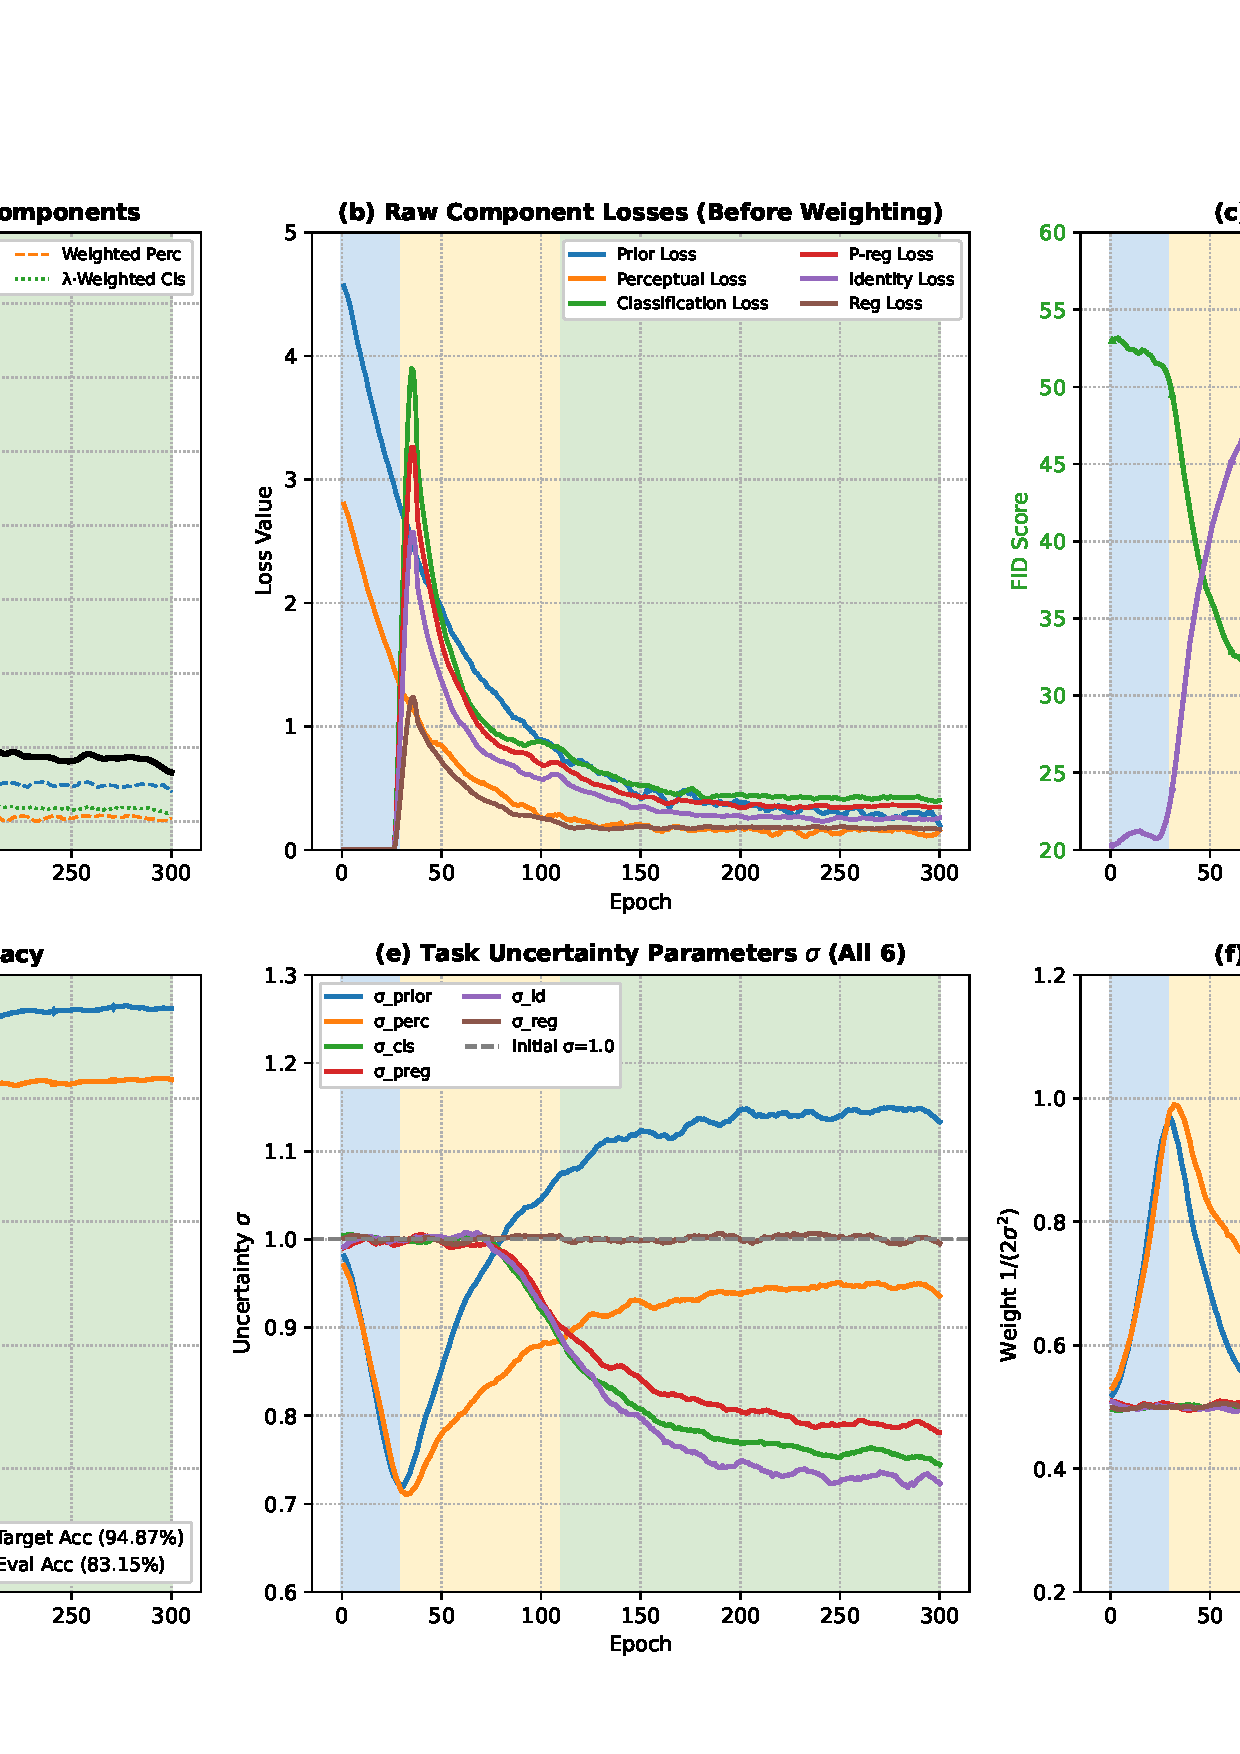
\includegraphics[width=\textwidth]{figures/mia_training_curves.pdf}
  \caption{模型反演方法三阶段渐进式训练过程的损失与指标演化曲线。(a)总损失与主要分项损失;(b)所有分项损失的演化;(c)目标准确率(Target Acc)和评估准确率(Eval Acc)的提升;(d)生成质量指标FID的下降和KNN距离的上升;(e)任务不确定性权重的自适应调整;(f)混合条件余弦退火系数$\lambda(t)$的平滑过渡。背景色区分三个训练阶段:阶段1(粉色)为图像条件预热,阶段2(蓝色)为混合条件过渡,阶段3(绿色)为纯标签条件适配。}
  \label{fig:mia_training_curves}
\end{figure}

% \subsubsection{LoRA配置消融}

% 表~\ref{tab:mia_lora_ablation}对比了不同LoRA秩配置与全参数微调的性能与效率。

% \begin{table}[htbp]
%   \centering
%   \caption{MIA低秩适应配置消融实验(VGGFace2 + ArcFace)}
%   \label{tab:mia_lora_ablation}
%   \begin{tabular}{lccccc}
%     \hline
%     LoRA配置 & Acc1 & FID & 可训练参数 & 训练时间 & GPU内存 \\
%     \hline
%     r=8 & 91.20\% & 25.15 & 0.8M (0.09\%) & 5.2h & 14.3GB \\
%     r=16 & 93.47\% & 23.82 & 1.5M (0.18\%) & 6.0h & 16.8GB \\
%     r=32 & 93.73\% & 23.64 & 2.9M (0.34\%) & 7.8h & 19.2GB \\
%     全参数微调 & 94.13\% & 23.21 & 856.2M (100\%) & 96h & 28.5GB \\
%     \hline
%   \end{tabular}
% \end{table}

% 实验结果展示了LoRA技术的参数效率优势。秩$r=16$时,仅训练0.18\%的参数(1.5M),即可达到93.47\%的攻击准确率和23.82的FID,与全参数微调(Acc1 94.13\%,FID 23.21)的性能差距极小。继续增加秩至32,性能提升不足0.3个百分点,但参数量翻倍。从训练效率看,LoRA相比全参数微调训练时间缩短16倍,GPU内存占用降低41\%。该结果验证了第四章选择$r=16$作为最佳配置的合理性,在参数效率与攻击性能之间达到最优平衡。

\subsubsection{损失项组合消融}

表~\ref{tab:mia_loss_ablation}展示了不同损失项组合对MIA性能的影响。

\begin{table}[htbp]
  \centering
  \caption{模型反演方法损失项组合消融实验(VGGFace2 + ArcFace)}
  \label{tab:mia_loss_ablation}
  \begin{tabular}{lcccc}
    \hline
    损失组合 & TarAcc & EvalAcc & FID & KNN Dist \\
    \hline
    仅扩散先验 $\mathcal{L}_{\text{prior}}$ & 7.85\% & 5.92\% & 53.47 & 0.4156 \\
    + 分类引导 $\mathcal{L}_{\text{cls}}$ & 77.24\% & 70.38\% & 36.82 & 0.5387 \\
    + 身份一致性 $\mathcal{L}_{\text{id}}$ & 92.56\% & 79.47\% & 29.15 & 0.6743 \\
    + 感知质量 $\mathcal{L}_{\text{perc}}$ & 94.87\% & 83.15\% & 23.26 & 0.7165 \\
    \hline
  \end{tabular}
\end{table}

实验结果表明各损失项的协同作用。仅使用扩散先验损失时,由于缺乏针对目标分类器的优化信号,目标准确率仅为7.85\%,评估准确率更低至5.92\%,FID高达53.47,KNN距离仅为0.4156。引入top-k max-margin分类引导损失后,通过直接优化目标类别置信度并远离决策边界,目标准确率显著提升至77.24\%,评估准确率提升至70.38\%,FID降至36.82,KNN距离提高到0.5387。进一步添加身份一致性损失,通过对比学习确保生成图像的身份特征与标签嵌入一致,目标准确率达到92.56\%,评估准确率达到79.47\%,FID进一步降至29.15,KNN距离提高到0.6743。最后引入LPIPS感知质量损失,在保持攻击有效性的同时优化视觉真实性,使目标准确率达到94.87\%,评估准确率达到83.15\%,FID降至23.26,KNN距离达到0.7165。值得注意的是,每增加一个损失项,评估准确率的提升幅度都大于目标准确率,特别是身份一致性损失带来了显著提升,表明这些损失项不仅提高了对目标模型的攻击成功率,更重要的是增强了生成样本的真实代表性和泛化能力,生成图像在特征空间中与真实样本的相似度显著提升。该结果验证了第四章提出的多目标优化框架的必要性,各损失项缺一不可。

\subsection{训练动态与收敛性分析}

为深入理解模型反演方法的学习过程,本节分析渐进式三阶段训练策略的动态特性。图~\ref{fig:mia_training_curves}展示了完整训练流程的损失演化和性能指标变化。

三阶段训练过程呈现出清晰的阶段性特征。图像条件预热阶段中,扩散先验损失$\mathcal{L}_{\text{prior}}$快速下降,标签嵌入层通过真实图像监督建立起有效的身份表示基础。混合条件过渡阶段中,随着余弦退火调度逐渐降低图像条件权重,分类引导损失$\mathcal{L}_{\text{cls}}$和身份一致性损失$\mathcal{L}_{\text{id}}$协同优化,目标准确率从接近0\%平滑上升至89\%,评估准确率提升至79\%,FID从初始的50+降至32左右,KNN距离提高到0.63左右。这一平滑过渡避免了直接切换到纯标签条件导致的训练崩塌。纯标签微调阶段中,模型在无图像监督下完成最终优化,目标准确率稳定在94.87\%,评估准确率达到83.15\%,FID降至23.26,KNN距离达到0.7165,验证了标签嵌入的泛化能力和生成样本的真实代表性。

任务不确定性加权机制在多目标平衡中发挥了关键作用。如图~\ref{fig:mia_training_curves}(e)所示,五个损失项的权重$1/\sigma_i^2$在训练过程中动态调整:扩散先验权重在阶段1保持主导地位,确保生成质量基础;分类引导权重在阶段2-3逐渐增强,驱动攻击准确率提升;感知质量权重$1/\sigma_{\text{perc}}^2$始终维持适度水平,在不牺牲攻击性能的前提下优化视觉真实性。这种自动权重调整机制使框架无需人工超参数搜索即可在五个优化目标间达到动态均衡。

\subsection{模型反演攻击方法实验小结}

本节通过系统实验验证了基于换脸先验迁移的多目标自适应模型反演方法的有效性与优越性。实验结果表明:(1)攻击准确率与代表性方面,本文方法在不同架构的目标分类器上均取得了显著优于现有方法的目标准确率和评估准确率,特别是在评估准确率上的提升证明了生成样本真正代表目标类别而非仅适配目标模型,展现了方法的跨架构泛化能力;(2)生成质量方面,FID、KNN距离等多维度指标均表明生成图像在分布一致性和特征接近度上达到了较高水平,其中更低的FID和更高的KNN距离反映了生成样本与真实数据的高度相似性;(3)核心技术方面,消融实验证实渐进式三阶段训练策略是实现从图像条件到标签条件平滑过渡的关键,LoRA参数高效微调在极少参数量下达到接近全参数微调的效果,任务不确定性加权框架自动平衡多个优化目标避免了繁琐的超参数调试;(4)可视化分析表明生成图像具有高身份一致性和视觉真实感。这些发现全面验证了本文提出的方法在模型反演攻击任务中的创新性与实用性。

\section[本章小结]{本章小结}
\label{sec:results_summary}

本章通过系统的实验验证了本文提出的模板逆向攻击与模型反演攻击方法的有效性,并对关键技术组件的作用进行了深入分析。

针对模板逆向攻击任务,实验结果表明第三章提出的基于角度约束对比学习的模板逆向重建方法在白盒场景下能够实现高成功率的模板重建。与现有方法相比,本文方法在攻击成功率上达到了更高的水平,同时保持了合理的生成质量。消融实验验证了角度约束特征匹配在超球面特征空间中的优势,任务不确定性加权机制能够自动平衡像素质量与特征匹配,而多样性正则化有效避免了模式崩塌问题。这些设计共同作用,使得方法能够从有限的模板向量生成高保真度的人脸图像。

针对模型反演攻击任务,实验证实了第四章提出的基于换脸先验迁移的多目标自适应模型反演方法在攻击准确率和生成保真度之间取得了良好的平衡。在VGGFace2数据集上训练的不同架构目标分类器上,方法均表现出稳定的性能,验证了跨架构的泛化能力。消融实验说明了渐进式三阶段训练策略的重要性,其通过逐步过渡实现了从图像条件到标签条件的平稳转换。LoRA参数高效微调技术使得方法仅需微调极少比例的参数就能达到接近全参数微调的效果,大幅降低了计算和存储开销。任务不确定性加权框架则自动平衡了扩散先验、分类引导、身份一致性、感知质量和正则化五个优化目标,避免了繁琐的超参数调试。

综上所述,本章实验全面验证了本文方法的有效性和泛化性。实验结果不仅展示了人脸识别系统面临的隐私泄露风险,也为防御机制的设计提供了实证依据。这些发现对于推动隐私保护技术的发展具有重要的理论和实践意义。

% Local Variables:
% TeX-master: "../main"
% TeX-engine: xetex
% End:
